\documentclass{article}

\usepackage{amsmath}
\usepackage{amssymb}

\usepackage{geometry}
\geometry{margin=1.5in}

\usepackage{graphicx}

\begin{document}

\textbf{What is a kernel?}

To classify, we need some measure of similarity. Let's define some function $k$
that takes two arguments $x$ and $x'$ and returns a real number expressing their
similarity:

$$
k: \mathcal{X} \times \mathcal{X} \rightarrow \mathbb{R}
$$

As an example, take the dot product.

$$
k(\mathbf{x}, \mathbf{x}') = \langle \mathbf{x}, \mathbf{x}' \rangle = \sum x_ix'_i
$$

\textit{Geometrically}, the dot product expresses the cosine of the angle
between $\mathbf{x}$ and $\mathbf{x}'$. The dot product also expresses the 
\textit{length} of a vector, i.e.
$||\mathbf{x}|| = \sqrt{\langle \mathbf{x}, \mathbf{x} \rangle}$. Lastly, the
\textit{distance} between two vectors is computed as the length of the difference vector.
So, being able to compute dot products amounts to being able to carry out all
mathematical operations that can be characterized in terms of angles, lengths,
and distances (cough cough, linear algebra and analytic geometry).

BUT, we cannot take for granted that our data actually lives in a
dot product space. For example, it might be text strings. So, we need some
transformation that takes possibly non-vectorial data $x$ and maps it to the dot
product space $\mathcal{H}$ (which need not be $\mathbb{R}^n$).

$$
\Phi: \mathcal{X} \rightarrow \mathcal{H}
$$
$$
x \mapsto \mathbf{x} := \Phi(x)
$$

We can cleverly pick our kernel function so that we do not actually need to
carry out this mapping.

\bigskip

\textbf{The ``kernel trick''}

Suppose that we have the feature map $\Phi$ that takes two-dimensional inputs and
maps them to a three-dimensional space.
$$
\Phi: \mathbb{R}^2 \rightarrow \mathbb{R}^3
$$
Specifically:
\begin{equation}
\Phi: \left[x_1, x_2 \right] \rightarrow \left[x_1^2, x_2^2, \sqrt{2}x_1x_2
\right]
\end{equation}

Now suppose that we will perform standard soft-margin SVM on the transformed
data. In its dual form:

$$
\max_{\alpha \in \mathbb{R}^n} 
\sum_{i=1}^n \alpha_i - \frac{1}{2} \sum_{i=0}^n \sum_{j=0}^n \alpha_i \alpha_j
Y_i Y_j \langle \Phi(X_i), \Phi(X_j) \rangle
$$

Let's examine that inner product bit on the right in more detail.

$$
\langle \Phi(X_i), \Phi(X_j) \rangle = \langle (X_{i1}^2, X_{i2}^2,
\sqrt{2}X_{i1}X_{j2}),  (X_{j1}^2, X_{j2}^2,
\sqrt{2}X_{i1}X_{j2})\rangle
$$
$$
= X_{i1}^2X_{j1}^2 + 2X_{i1}X_{i_2}X_{j1}X_{j2} + X_{i2}^2X_{j2}^2
$$
$$
= (X_{i1}X_{j1} + X_{j1}X_{j2})^2
$$
$$
= \langle X_i, X_j \rangle^2
$$
$$
:= k(x, x')
$$

(i.e. we are defining our kernel function to be the inner product, squared). Now we rewrite our SVM:

$$
\max_{\alpha \in \mathbb{R}^n} 
\sum_{i=1}^n \alpha_i - \frac{1}{2} \sum_{i=0}^n \sum_{j=0}^n \alpha_i \alpha_j
Y_i Y_j k(X_i, X_j)
$$

Note that we are operating directly on the untransformed $X$, i.e. without
having to conduct the transformation $\Phi$. We have defined $k$ such that $k(x,
x') = \langle \Phi(x), \Phi(x') \rangle$. This is the \textbf{kernel trick}.
It works for any kernel function $k$ that is symmetric and positive
semi-definite. Some common such kernels are:
\begin{itemize}
\item Linear: $k(x, x') = \langle x, x' \rangle$
\item Polynomial: $k(x, x') = \langle x, x' \rangle^\gamma$
\item Gaussian (RBF): $k(x, x') = \exp(-\frac{||x - x'||^2_2}{2\sigma^2})$. This
is the de facto standard for machine learning.
\end{itemize}

\bigskip

\textbf{Why do we care?}

The kernel trick, and kernel methods in general, have some nice value
propositions.

The first is \textbf{applying linear methods to non-linear problems}. Choosing a
kernel that lets us map between dimensions can allow us to apply linear methods
when we otherwise wouldn't be able to. Consider the below classification
problem. Clearly, the best decision boundary is an ellipse, which is non-linear,
so we cannot apply something like SVM. But if we map $\mathbb{R}^2$ to
$\mathbb{R}^3$ using (1), we can train a SVM to separate the classes.

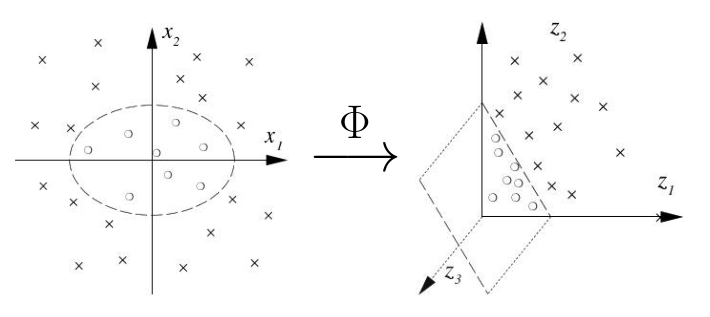
\includegraphics[scale=0.5]{kernel}

Similarly, we can use kernels to apply machine learning methods to non-vectorial
data such as text strings or k-grams or labelled graphs.

The second is \textbf{computational efficiency}. Because of the kernel trick
(and some other stuff covered later), we can explore enormous features spaces
for classification purposes without actually computing such spaces. Suppose we
have $d=100$ and want to consider up to 3rd degree interactions. This already
leads to $d=171,700$---not trivial to compute! Yet through the kernel trick, we
do not actually need to conduct the laborious mapping $\Phi$, we can operate
directly on the input data through the kernel. 

\newpage

\textbf{Reproducing kernel Hilbert spaces and the representer theorem}

HOLY SHIT THIS IS ABSTRACT

As previously covered, a Hilbert space basically is one where we have the dot
product. 

Reproducing property:

$$
\langle k(x, \bullet), k(x', \bullet) \rangle_{\mathcal{H}_k} := k(x, x')
$$

\end{document}
